\chapter{Background and Related Work}\label{ch:related}
\section{Influence maximization and diffusion}
An influence-maximization objective depends on how activation spreads. The Independent Cascade model assigns transmission opportunities to newly active nodes, with edge-specific success probabilities. Expected final spread can then define a set function over seeds. The classical analysis of Kempe, Kleinberg, and Tardos establishes computational hardness and exploits monotonicity and submodularity for approximation in appropriate diffusion models \cite{kempe2003}. These results explain why the marginal benefit of a seed, rather than its degree alone, matters.

Efficient seed selection must account for overlap. Two high-degree seeds may reach nearly the same neighborhood. CELF uses lazy evaluation of marginal gains to reduce repeated work in greedy submodular selection \cite{leskovec2007}. The saved CELF result in this project is a reference denominator, not a proof that the learned model reaches a fixed fraction of a globally optimal solution. A ratio to a heuristic reference should not be confused with a fraction of all vertices.

The project deliberately uses one-step outgoing IC with transmission probability one. Its spread is the size of the union of the selected seeds and their outgoing neighbors. This is a deterministic coverage objective for a fixed graph and seed set. Multi-hop stochastic cascades raise additional issues not tested by the current evaluation. The distinction is important because a mechanism can behave differently under long-range propagation, repeated diffusion simulation, or edge probabilities below one.

\subsection{From cascade reachability to a coverage function}
The live-edge representation gives a common description of the general IC objective and its one-step specialization \cite{kempe2003,hou2025}. For every directed edge $(u,v)$, draw an independent Bernoulli variable with success probability $w_{uv}$. Keep the edge when the draw succeeds. A later activation attempt can then use the draw already associated with that edge. With an unrestricted horizon, the final active vertices are precisely those reachable from at least one seed in the resulting graph. With a horizon of $h$ steps, take only paths of length at most $h$. In both cases a path of length zero includes the seed itself.

For a fixed realization $\omega$, write $R_{\omega,h}(v)$ for the vertices reachable from $v$ within the horizon. The spread $F_{\omega,h}$ and the gain from adding $v$ are
\begin{align}
 F_{\omega,h}(S)
 &=\left|\bigcup_{s\in S}R_{\omega,h}(s)\right|,\\
 F_{\omega,h}(S\cup\{v\})-F_{\omega,h}(S)
 &=\left|R_{\omega,h}(v)\setminus\bigcup_{s\in S}R_{\omega,h}(s)\right|.
\end{align}
Enlarging $S$ can only shrink the set counted in the second line. The gain is nonnegative and decreases weakly as the seed set grows. Both inequalities hold for every realization and therefore also hold after taking expectations. In the thesis evaluation, $h=1$ and every tested edge is live with probability one, so $R_{\omega,1}(v)=\{v\}\cup N^+(v)$ is fixed. This reduces the probability model to the closed outgoing-neighborhood union used in Chapter~\ref{ch:problem}.

Lazy greedy evaluation exploits the same inequality. If the gain of a candidate was last computed for a smaller seed set, that value is an upper bound for its current gain. A candidate with an older upper bound above the best recomputed value may still require a fresh evaluation. Once the best recomputed gain is at least all remaining upper bounds, the next greedy choice is determined up to ties. The acceleration changes how the greedy choice is found. Its output is still a set produced by a sequence of marginal comparisons under the fixed reference protocol \cite{leskovec2007}.

\subsection{Redundancy among high-scoring candidates}
Consider an illustrative directed graph with vertices $a,b,c,x,y,z,u,w$. The arcs from each of $a$ and $b$ point to $x,y,z$. The arcs from $c$ point to $u,w$. All other vertices have no outgoing edges. For the one-step objective, the singleton spreads of $a,b,c$ are $4,4,3$. Ranking once by singleton spread and taking the first two selects $a,b$, which cover five vertices because their three reachable neighbors coincide. Selecting $a,c$ covers seven. With $\{a\}$ already selected, the marginal gain of $b$ is one, whereas the marginal gain of $c$ is three.

\begin{figure}[htbp]
\centering
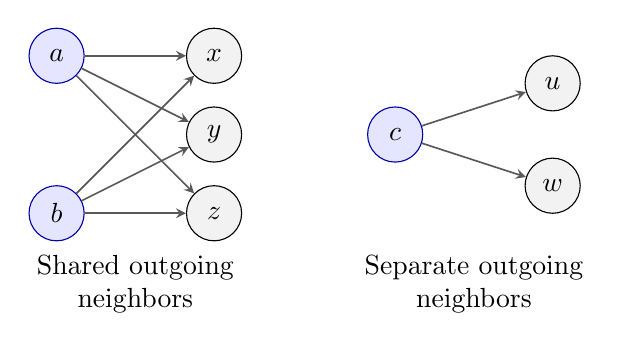
\begin{tikzpicture}[
 x=1cm,y=1cm,
 vertex/.style={circle,draw,minimum size=7mm,inner sep=0pt},
 seed/.style={vertex,draw=blue!65!black,fill=blue!10},
 reached/.style={vertex,fill=black!5},
 arc/.style={->,>=stealth,semithick,draw=black!65}]
 \node[seed] (a) at (0,2) {$a$};
 \node[seed] (b) at (0,0) {$b$};
 \node[reached] (x) at (2,2) {$x$};
 \node[reached] (y) at (2,1) {$y$};
 \node[reached] (z) at (2,0) {$z$};
 \node[seed] (c) at (4.3,1) {$c$};
 \node[reached] (u) at (6.3,1.65) {$u$};
 \node[reached] (w) at (6.3,0.35) {$w$};
 \foreach \source in {a,b}
   \foreach \destination in {x,y,z}
     \draw[arc] (\source) -- (\destination);
 \draw[arc] (c) -- (u);
 \draw[arc] (c) -- (w);
 \node[align=center] at (1,-0.9) {Shared outgoing\\neighbors};
 \node[align=center] at (5.3,-0.9) {Separate outgoing\\neighbors};
\end{tikzpicture}
\caption[Overlapping and complementary seed neighborhoods]{Illustrative graph for one-step spread. Selecting $a$ and $b$ covers five vertices. Selecting $a$ and $c$ covers seven.}
\label{fig:seed-overlap}
\end{figure}

Figure~\ref{fig:seed-overlap} shows the information a scoring model needs to act as a useful surrogate for set selection. A scoring map that reads the graph can use information beyond a node's degree. Since the final Top-$k$ rule chooses individual scores in one pass, the model has to encode any preference for complementary candidates in those scores. Greedy CELF can recompute the benefit of each candidate conditional on the seeds chosen so far.

\section{Learning structural influence scores}
A GNN replaces repeated combinatorial decisions with a learned map from graph structure to scores. Message passing can represent structural interactions, while a differentiable objective can encourage a useful covering set. FastCover introduces an unsupervised framework with a graph reversed attention network, GRAT, and obtains a seed set from learned node scores \cite{ni2021}. This provides architectural context for the released GRAT components inherited by the present project.

PrivIM specifically studies private GNN-based influence maximization and includes Sensitivity-Constrained Sampling and Boundary-Enhanced Sampling \cite{hou2025}. The current reproduction retains those sampling components within each stable slot. Its private mechanism, however, uses a separately documented locality argument: fixed slot membership bounds the number of affected slot contributions, each of which is clipped. The dissertation does not import a historical privacy claim merely because the same sampling function is called. The frozen accountant and adjacency definition must match the query that is actually trained.

There is also a reproduction distinction between the architecture in a mathematical appendix and a released implementation. The current runs use the legacy released GRAT layer, with biased linear maps and attention computed from pre-transformation node features. They do not use the separately available paper-appendix variant. All four final configurations retain that model identity. A different attention activation, feature construction, or parameterization would change the experiment and cannot silently be substituted when explaining results.

The thesis thus builds on existing GNN influence scoring and PrivIM components. It does not claim to introduce the first GNN influence maximizer or the first node-private influence-maximization method. Its question concerns whether a particular heterogeneous node policy, applied through a frozen training mechanism, produces a reliable utility gain against a strict uniform control.

\section{Differential privacy and private optimization}
Differential privacy bounds how much the output distribution can change between neighboring datasets. Its parameters describe a probabilistic relation between distributions rather than the amount of information an attacker happened to recover in a particular test. Postprocessing and composition provide essential design rules \cite{dwork2014}. The adjacency relation remains indispensable: a guarantee about changing one edge is different from a guarantee about adding or removing a node and all its incident edges.

DP-SGD develops private neural optimization using bounded gradient contributions, noise, and a privacy accountant \cite{abadi2016}. On ordinary records, the contribution unit is comparatively direct. A graph violates the naive analogy between one node and one independently affected gradient because a node may appear in many subgraphs and affect neighboring representations. The present mechanism therefore clips both individual position gradients and their slot sums. This is a structural sensitivity construction in addition to a numerical norm restriction.

R\'enyi differential privacy (RDP) bounds the divergence between output distributions on adjacent inputs. For probability laws $P$ and $Q$ with $P$ absolutely continuous with respect to $Q$, the order-$\alpha$ R\'enyi divergence is
\begin{equation}
 D_\alpha(P\|Q)=\frac{1}{\alpha-1}
 \log \mathbb{E}_{X\sim Q}\!\left[\left(\frac{dP}{dQ}(X)\right)^\alpha\right],
 \qquad \alpha>1.
\end{equation}
The divergence is infinite when $P$ is not absolutely continuous with respect to $Q$. A mechanism is $(\alpha,\rho)$-RDP if this divergence is at most $\rho$ for its output laws on every ordered pair of adjacent inputs \cite{mironov2017}. At a fixed order $\alpha$, bounds that hold conditional on every common output history add across adaptive updates. Chapter~\ref{ch:method} applies this rule to the full Gaussian training transcript before converting the resulting bound to $(\epsilon,\delta)$-DP.

Privacy amplification by subsampling requires a precise sampling model and compatible adjacency. Balle, Barthe, and Gaboardi analyze amplification using couplings and divergences \cite{balle2018}. In this project, the additional personalized amplification is applied once to the complete base training mechanism, because each node's outer participation is drawn once before training. The inner RWR/SCS/BES procedure is not counted as an extra unproved amplification factor.

\section{Node-private graph neural networks}
Prior node-private GNN research demonstrates that graph dependencies need explicit treatment. Daigavane et al. analyze node-private learning with sensitivity and graph-aware amplification \cite{daigavane2021}. GAP separates encoding, private aggregation, and classification, with edge- and node-level protection analyzed for its defined pipeline \cite{sajadmanesh2023}. DPAR decouples feature projection and message passing using privately computed approximate Personalized PageRank neighborhoods \cite{zhang2024}. Xiang et al. use HeterPoisson sampling to construct batches of subgraphs and symmetric multivariate Laplace noise for node-private GNN training \cite{xiang2024}. In PDP-PrivIM, stable slots and slot-level clipping bound the effect of removing a node before Gaussian perturbation.

These examples protect different computations from the current influence-ranking task. Their guarantees cannot be transferred by relabeling a loss or replacing a classifier with Top-50 ranking. Each method controls how protected graph information enters its queries and subsequent inference. The present stable-slot mechanism instead bounds arbitrary within-slot changes after node removal, while retaining the original subgraph-based objective inside each slot.

This comparison also distinguishes two meanings of ``personalized.'' Personalized PageRank concerns a graph-walk starting distribution; it does not inherently assign different DP budgets to people. Personalized prediction or federated model adaptation likewise need not imply personalized privacy requirements. The relevant policy in this dissertation is an explicit per-identity upper-bound vector, held fixed across neighboring graph inputs.

\section{Personalized privacy in graph learning}
Jorgensen et al. formulate personalized differential privacy and show how to use record-specific sampling probabilities to accommodate heterogeneous privacy requirements \cite{jorgensen2015}. Subsequent work also studies personalized privacy in GNNs. Yuan et al.'s PDPGNN assigns budgets using node degree and employs weighted aggregation \cite{yuan2026}. It addresses degree-dependent utility degradation. The present project instead fixes an external public Registry with target classes 1, 2, and 4 and uses one-time participation to meet those requirements. Its policy is not recomputed from the changing private degree sequence.

He et al. propose PPGNN for decentralized local graph data, combining personalized local perturbation with a weighted calibration strategy \cite{he2026}. That trust model differs from central private training over a fixed prepared graph. The paper is cited here in its verifiable arXiv form; its repository note about IEEE TKDE is not treated as independently verified final publication metadata. Its existence reinforces that the broad combination of personalization and graph privacy is not itself a first-of-its-kind claim.

This study combines a fixed target policy, stable overlapping slots, and full-coordinate training for influence maximization, and reports an exploratory evaluation of Coverage and run-to-run variability. PDPGNN and PPGNN provide context for the comparison of privacy models and training designs.

\section{High-dimensional optimization and stability}
A Gaussian mechanism can have a sensitivity bound independent of parameter count while injecting noise in every coordinate. If $Z\sim\mathcal{N}(0,\sigma^2 I_d)$, then $\E\|Z\|_2^2=d\sigma^2$. This elementary identity helps explain why the geometry of private optimization deserves attention. It does not imply that the same scaling holds for errors in logits or Coverage, which are nonlinear functions of the learned parameters and graph.

The current mechanism trains 2340 coordinates; a historical frozen-backbone comparator trains only 33. Their common per-coordinate scale can coexist with very different total parameter-space noise energy and clipping behavior. Historical results make that distinction worth investigating but do not isolate it causally. Different trainable subspaces, signal directions, and independent secret trajectories change together.

A small standard deviation can coexist with consistently poor utility, while a high mean can conceal severe losses in some runs. This dissertation therefore reports mean Coverage, sample SD, minima, maxima, and the frequency of Coverage below 50\%.

\section{Position of the present research}
The reviewed literature supplies the IM formulation, GRAT architecture, PrivIM sampling, RDP, and privacy amplification tools. The project combines these within a fixed-domain personalized node-private training design. The conditional privacy theorem applies to the specified model output under the assumptions stated in Chapter~\ref{ch:method}. The empirical analysis compares observed mean Coverage and run-to-run variability across the reported development configurations on five fixed datasets.
